\documentclass[11pt,compress,t,notes=noshow, xcolor=table]{beamer}

\usepackage[]{graphicx}\usepackage[]{color}
% maxwidth is the original width if it is less than linewidth
% otherwise use linewidth (to make sure the graphics do not exceed the margin)
\makeatletter
\def\maxwidth{ %
  \ifdim\Gin@nat@width>\linewidth
    \linewidth
  \else
    \Gin@nat@width
  \fi
}
\makeatother



\definecolor{fgcolor}{rgb}{0.345, 0.345, 0.345}
\newcommand{\hlnum}[1]{\textcolor[rgb]{0.686,0.059,0.569}{#1}}%
\newcommand{\hlstr}[1]{\textcolor[rgb]{0.192,0.494,0.8}{#1}}%
\newcommand{\hlcom}[1]{\textcolor[rgb]{0.678,0.584,0.686}{\textit{#1}}}%
\newcommand{\hlopt}[1]{\textcolor[rgb]{0,0,0}{#1}}%
\newcommand{\hlstd}[1]{\textcolor[rgb]{0.345,0.345,0.345}{#1}}%
\newcommand{\hlkwa}[1]{\textcolor[rgb]{0.161,0.373,0.58}{\textbf{#1}}}%
\newcommand{\hlkwb}[1]{\textcolor[rgb]{0.69,0.353,0.396}{#1}}%
\newcommand{\hlkwc}[1]{\textcolor[rgb]{0.333,0.667,0.333}{#1}}%
\newcommand{\hlkwd}[1]{\textcolor[rgb]{0.737,0.353,0.396}{\textbf{#1}}}%
\let\hlipl\hlkwb

\usepackage{framed}
\makeatletter
\newenvironment{kframe}{%
 \def\at@end@of@kframe{}%
 \ifinner\ifhmode%
  \def\at@end@of@kframe{\end{minipage}}%
  \begin{minipage}{\columnwidth}%
 \fi\fi%
 \def\FrameCommand##1{\hskip\@totalleftmargin \hskip-\fboxsep
 \colorbox{shadecolor}{##1}\hskip-\fboxsep
     % There is no \\@totalrightmargin, so:
     \hskip-\linewidth \hskip-\@totalleftmargin \hskip\columnwidth}%
 \MakeFramed {\advance\hsize-\width
   \@totalleftmargin\z@ \linewidth\hsize
   \@setminipage}}%
 {\par\unskip\endMakeFramed%
 \at@end@of@kframe}
\makeatother

\definecolor{shadecolor}{rgb}{.97, .97, .97}
\definecolor{messagecolor}{rgb}{0, 0, 0}
\definecolor{warningcolor}{rgb}{1, 0, 1}
\definecolor{errorcolor}{rgb}{1, 0, 0}
\newenvironment{knitrout}{}{} % an empty environment to be redefined in TeX

\usepackage{alltt}
\newcommand{\SweaveOpts}[1]{}  % do not interfere with LaTeX
\newcommand{\SweaveInput}[1]{} % because they are not real TeX commands
\newcommand{\Sexpr}[1]{}       % will only be parsed by R
\newcommand{\xmark}{\ding{55}}%


\usepackage[english]{babel}
\usepackage[utf8]{inputenc}

\usepackage{dsfont}
\usepackage{verbatim}
\usepackage{amsmath}
\usepackage{amsfonts}
\usepackage{amssymb}
\usepackage{bm}
\usepackage{csquotes}
\usepackage{multirow}
\usepackage{longtable}
\usepackage{booktabs}
\usepackage{enumerate}
\usepackage[absolute,overlay]{textpos}
\usepackage{psfrag}
\usepackage{algorithm}
\usepackage{algpseudocode}
\usepackage{eqnarray}
\usepackage{arydshln}
\usepackage{tabularx}
\usepackage{placeins}
\usepackage{tikz}
\usepackage{setspace}
\usepackage{colortbl}
\usepackage{mathtools}
\usepackage{wrapfig}
\usepackage{bm}
\usepackage{amsmath}
\usepackage{pifont}

\usetikzlibrary{shapes,arrows,automata,positioning,calc,chains,trees, shadows}
\tikzset{
  %Define standard arrow tip
  >=stealth',
  %Define style for boxes
  punkt/.style={
    rectangle,
    rounded corners,
    draw=black, very thick,
    text width=6.5em,
    minimum height=2em,
    text centered},
  % Define arrow style
  pil/.style={
    ->,
    thick,
    shorten <=2pt,
    shorten >=2pt,}
}

\usepackage{subfig}

% Defines macros and environments
\usepackage{../../style/lmu-lecture}


\let\code=\texttt
\let\proglang=\textsf

\setkeys{Gin}{width=0.9\textwidth}

\setbeamertemplate{frametitle}{\expandafter\uppercase\expandafter\insertframetitle}

% This file is included in slides and exercises

% Rarely used fontstyle for R packages, used only in 
% - forests/slides-forests-benchmark.tex
% - exercises/single-exercises/methods_l_1.Rnw
% - slides/cart/attic/slides_extra_trees.Rnw
\newcommand{\pkg}[1]{{\fontseries{b}\selectfont #1}}

% Spacing helpers, used often (mostly in exercises for \dlz)
\newcommand{\lz}{\vspace{0.5cm}} % vertical space (used often in slides)
\newcommand{\dlz}{\vspace{1cm}}  % double vertical space (used often in exercises, never in slides)
\newcommand{\oneliner}[1] % Oneliner for important statements, used e.g. in iml, algods
{\begin{block}{}\begin{center}\begin{Large}#1\end{Large}\end{center}\end{block}}

% Don't know if this is used or needed, remove?
% textcolor that works in mathmode
% https://tex.stackexchange.com/a/261480
% Used e.g. in forests/slides-forests-bagging.tex
% [...] \textcolor{blue}{\tfrac{1}{M}\sum^M_{m} [...]
% \makeatletter
% \renewcommand*{\@textcolor}[3]{%
%   \protect\leavevmode
%   \begingroup
%     \color#1{#2}#3%
%   \endgroup
% }
% \makeatother






\title{Introduction to Machine Learning}

\begin{document}

\titlemeta{% Chunk title (example: CART, Forests, Boosting, ...), can be empty
  Classification
  }{% Lecture title  
  Tasks
}{% Relative path to title page image: Can be empty but must not start with slides/
  figure/tasks-bc.png
}{% Learning goals, wrapped inside itemize environment
  \item Understand the main difference between regression and classification
  \item Know that classification can be binary or multiclass
  \item Know some examples of classification tasks
}

\begin{vbframe}{Classification}
Learn functions that assign class labels to observation / feature vectors. Each observation belongs to exactly one class. The main difference to regression is the scale of the output / label.
{\centering \includegraphics[width= .7\textwidth]{figure_man/classifier.pdf}}

\end{vbframe}

\begin{vbframe}{Binary and Multiclass Tasks}
The task can contain two classes (\textbf{binary}) or multiple (\textbf{multiclass}).

\vspace{1em}

\begin{center}
\includegraphics[width=\textwidth]{figure/tasks-combined.png}
\end{center}

However, binary classification methods \textit{can} be effectively adapted for multiclass problems using decomposition techniques!

\end{vbframe}


\begin{vbframe}{Binary Classification Task - Examples}

  \begin{itemize}
  \item Credit risk prediction, based on personal data and transactions
  \item Spam detection, based on textual features
  \item Churn prediction, based on customer behavior
  \item Predisposition for specific illness, based on genetic data
  % \item $\ldots$
\end{itemize}

\begin{center}
  % FIGURE SOURCE: https://docs.google.com/presentation/d/1X2FxetT6fewXhoGLZmgJyEHY_pWbKjQ6AHZiZQHvwzA/edit?usp=sharing
  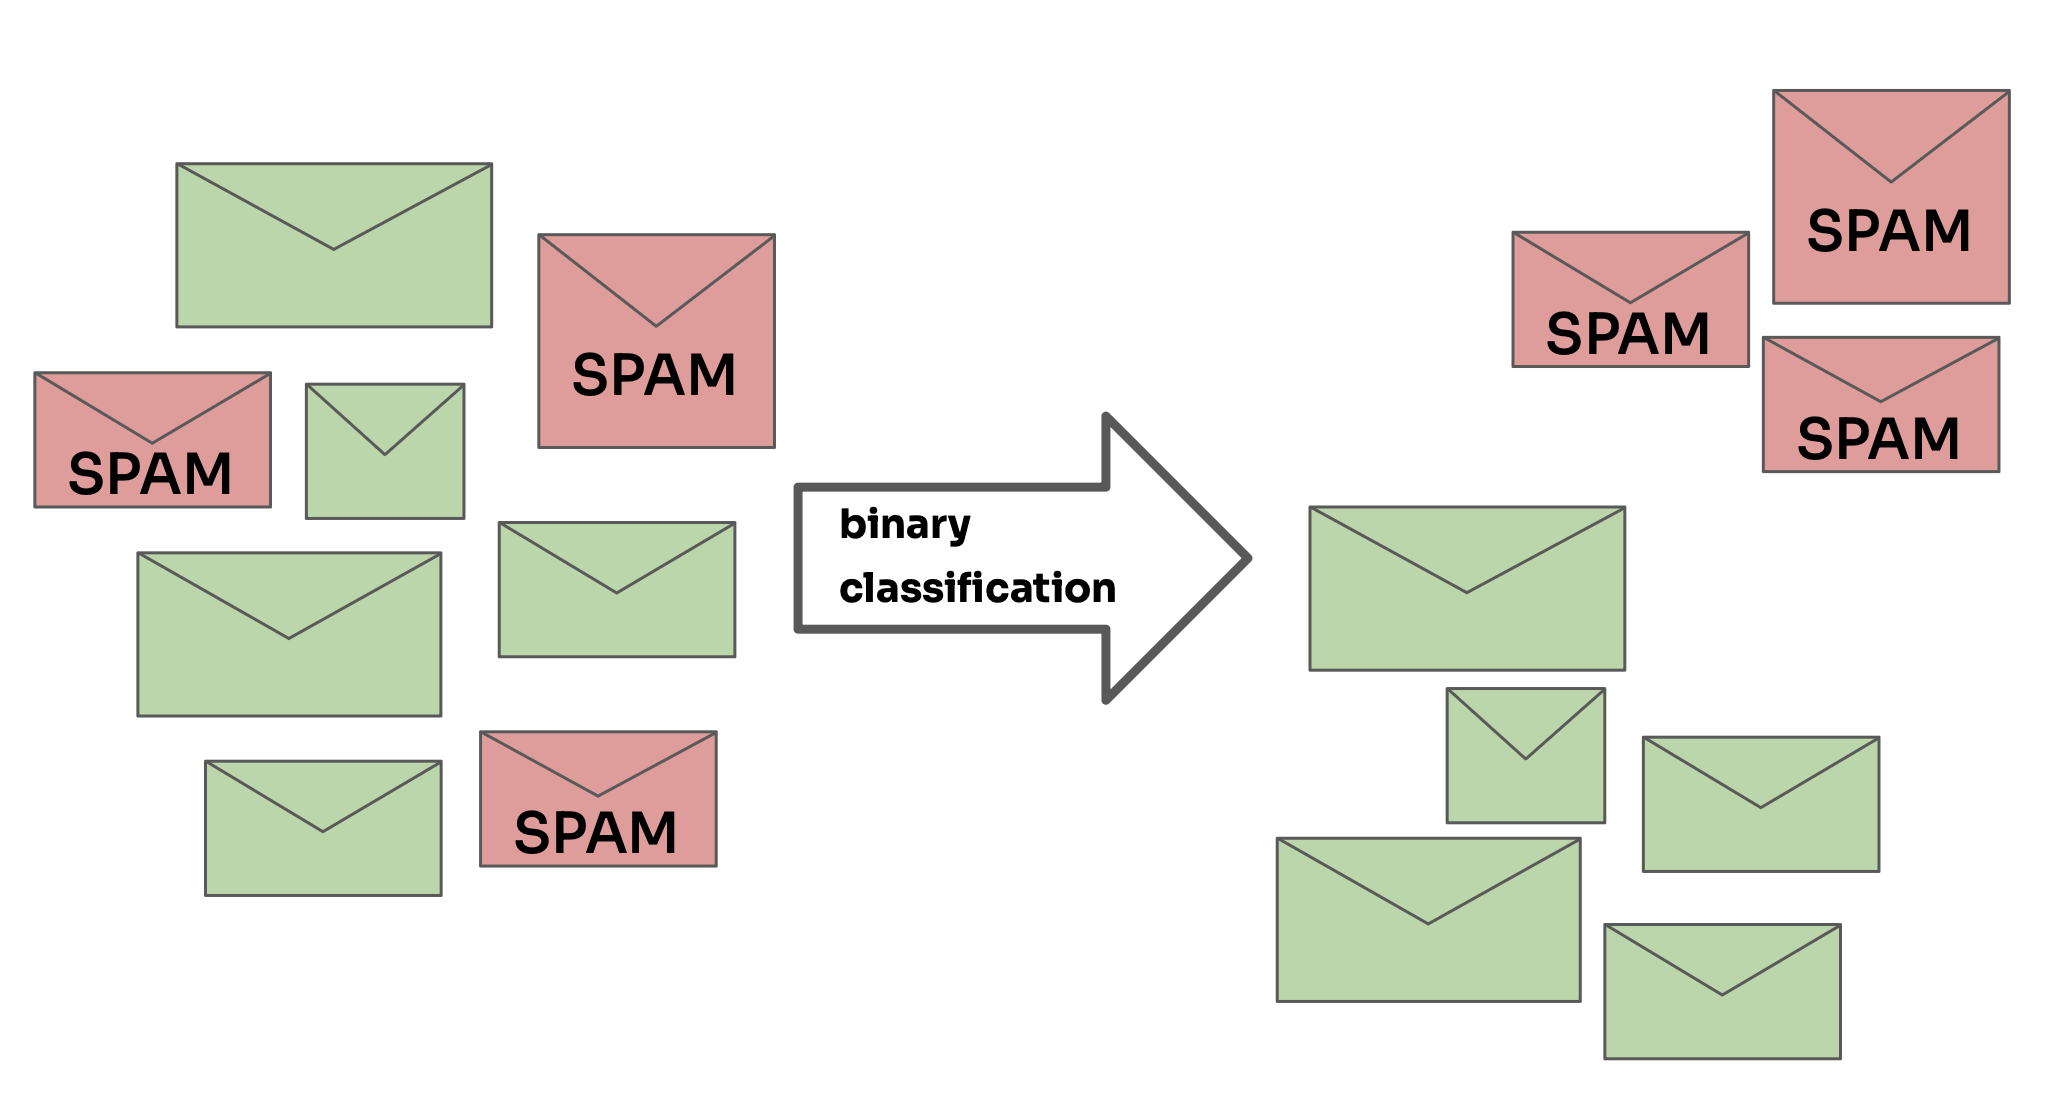
\includegraphics[width=0.9\textwidth]{figure_man/spam.png}
\end{center}
\end{vbframe}



\begin{vbframe}{Multiclass Task - Medical Diagnosis}
\begin{center}
  % FIGURE SOURCE: https://symptoms.webmd.com
  \includegraphics[width=0.8\textwidth]{figure_man/webmd.png}
\end{center}
\vspace{-0.5cm}
\begin{flushright}
  \tiny https://symptoms.webmd.com
\end{flushright}
\end{vbframe}

\begin{vbframe}{Multiclass Task - Iris}

The iris dataset was introduced by the statistician Ronald Fisher and is one
of the most frequent used data sets. Originally, it was designed for linear
discriminant analysis.

\begin{center}
\parbox{0.3\textwidth}{
\centering
  \begin{tabular}{@{}c@{}}
    \includegraphics[width=0.25\textwidth]{figure_man/iris_setosa.jpg} \\[\abovecaptionskip]
    \small Setosa
  \end{tabular}
}
\parbox{0.3\textwidth}{
\centering
  \begin{tabular}{@{}c@{}}
    \includegraphics[width=0.25\textwidth]{figure_man/iris_versicolor.jpg} \\[\abovecaptionskip]
    \small Versicolor
  \end{tabular}
}
\parbox{0.3\textwidth}{
\centering
  \begin{tabular}{@{}c@{}}
    \includegraphics[width=0.25\textwidth]{figure_man/iris_virginica.jpg} \\[\abovecaptionskip]
    \small Virginica
  \end{tabular}
}
\end{center}
  Source: \url{https://en.wikipedia.org/wiki/Iris\_flower\_data\_set}
\end{vbframe}

\begin{vbframe}{Multiclass Task - Iris}

\begin{columns}[T]
\begin{column}{0.5\textwidth}
\begin{itemize}
\item 150 iris flowers
\item Predict subspecies
\item Based on sepal and petal length / width in [cm]
\end{itemize}
\end{column}
\begin{column}{0.5\textwidth}
\includegraphics[width=0.4\textwidth]{figure_man/iris_petal_sepal.png}
\end{column}
\end{columns}
{\scriptsize
\begin{verbatim}
##      Sepal.Length Sepal.Width Petal.Length Petal.Width   Species
##   1:          5.1         3.5          1.4         0.2    setosa
##   2:          4.9         3.0          1.4         0.2    setosa
##   3:          4.7         3.2          1.3         0.2    setosa
##   4:          4.6         3.1          1.5         0.2    setosa
##   5:          5.0         3.6          1.4         0.2    setosa
##  ---
## 146:          6.7         3.0          5.2         2.3 virginica
## 147:          6.3         2.5          5.0         1.9 virginica
## 148:          6.5         3.0          5.2         2.0 virginica
## 149:          6.2         3.4          5.4         2.3 virginica
## 150:          5.9         3.0          5.1         1.8 virginica
\end{verbatim}
}
\end{vbframe}

\begin{vbframe}{Multiclass Task - Iris}
\begin{knitrout}\scriptsize
\definecolor{shadecolor}{rgb}{0.969, 0.969, 0.969}\color{fgcolor}

{\centering \includegraphics[width=0.95\textwidth]{figure/reg_class_task_3}

}

\end{knitrout}
\end{vbframe}


\endlecture

\end{document}
